\documentclass[12pt]{article}
\usepackage{amsmath}
\usepackage{amsfonts}
\usepackage{geometry}
\usepackage{graphicx}
\usepackage{setspace}
\usepackage{parskip}
\usepackage{hyperref}
\usepackage{graphicx}
\usepackage{float}
\usepackage{booktabs}
\newcommand{\comm}[1]{def}

\geometry{a4paper, margin=1in}
\setstretch{1.2}

\title{\Huge Orderbook Delta price reaction research}
\author{}
\date{}





    


\begin{document}

\maketitle


\subsection*{Table of Contents}

\begin{itemize}
  \item Outlier Detection Using Mean and Standard Deviation (Z-Score Based Outlier Detection)
  \item Measuring Volatility After Price Outlier Detection
  \item Measuring avearge return after price outlier detection
  \item Combining Indicators
\end{itemize}


\newpage

\section*{Outlier Detection Using Mean and Standard Deviation (Z-Score Based Outlier Detection)}


\subsection*{Normal Range}

What I want to test is how price reacts to anomalous orderbook delta movements, particularly in scenarios where unrealistic or clearly outlying values are detected. In cryptocurrency markets, such inefficiencies can be caused by various events, one example is liquidation
 events that interact with passive demand order stacked zones. During these events, the orderbook delta exhibits significant increases, providing a clear signal of market stress. This research will focus on understanding the relationship between rapid delta movements and how price reacts after these events.

\subsection*{My Hypothesis}

\begin{itemize}
  \item I expext realized volatility to increase after an outlier is detected. 
  \item I expext a return to the mean after a strong outlier is detected.
\end{itemize}



\subsection*{Normal Range}





\[
\mu(\Delta) \pm 2\sigma(\Delta)
\]

This means most data points (about 95\% if normally distributed) are expected to lie within this range.

\newpage

\subsection*{Outlier Condition}

A value is considered an outlier if:



\begin{equation}\label{eq: outlier_detection}
  \Delta < \mu(\Delta) - 2\sigma(\Delta) \quad \text{or} \quad \Delta > \mu(\Delta) + 2\sigma(\Delta)    
\end{equation}

This is a simple Z-score based outlier detection.

\begin{itemize}
  \item $\Delta$ - Orderbook Delta Depth with a certain depth I will test on: $\Delta_{1\%}$ $\Delta_{2.5\%}$ $\Delta_{5\%}$ from Coinbase (BTC/USD) 
  \item   This basically means we take a delta of the Bid and Ask orders which are in a range of x\% from the current price.
  \item $\mu(\Delta)$ — Mean of the last 1440 values of $\Delta$ before time $t$
  \item $\sigma(\Delta)$ - Standard deviation over the last 1440 $\Delta$ values before time $t$

\end{itemize}










\newpage


\subsection*{Idea behind}

\begin{itemize}
    \item This method assumes data is roughly normally distributed.
    \item Using $2\sigma$ captures approximately 95\% of data points under a normal distribution.
    \item You can adjust the multiplier (e.g., $3\sigma$) for stricter or looser thresholds.
\end{itemize}





\subsection*{Future Plans}

\begin{itemize}
    \item Test on more data
    \item use rolling windows (e.g. 1 day or 1 week) for local context.
    \item Compare sensitivity with +- 1.5$\sigma$ or +-2.5$\sigma$ $\rightarrow$ optimize for best results
\end{itemize}
















\newpage





\section*{Measuring Volatility After Price Outlier Detection}


\begin{equation}\label{eq:price_return}
    r_t = \frac{P_{t} - P_{t-1}}{P_{t-1}}
\end{equation}


\subsection*{Dictionary of Terms}

\begin{itemize}
    \item $P_t$  
      Asset price at time $t$.
    \item $r_t = \dfrac{P_t - P_{t-1}}{P_{t-1}}$  
      – 1-minute price return at time $t$.
    \item $\sigma^{\mathrm{(15)}}_{t}$  
      – Realized volatility: the standard deviation of the next 15 one-minute returns,
      
      

      
      \begin{equation}\label{eq:realized-vol}
        \sigma^{\mathrm{(15)}}_{t}
        = \sqrt{\frac{1}{14}\sum_{i=1}^{15}\bigl(r_{t+i}-\bar r_{t}\bigr)^{2}},
        \quad
        \bar r_{t} = \frac{1}{15}\sum_{i=1}^{15} r_{t+i}.
      \end{equation}
      



      aligned so that at time $t$ it measures volatility over $t+1$ to $t+15$.
\end{itemize}



\subsection*{In Python code}

\begin{verbatim}
import pandas as pd
df = pd.read_csv(file_path)
df.set_index('timestamp', inplace=True)
#Compute 1-min return of delta_5

df['r_t'] = df['price'].pct_change().fillna(0)


#compute rolling std of the future 15 min window

window = 15

#rolling on r_t, then shift forward so index t hold vol of t+1...t+15
df['future_vol_15] = (
    df['r_t']
    .rolling(window=window)
    .std()
    .shift(-window)
)
\end{verbatim}



\newpage

\subsection*{\textbf{Statistical evidence}}

Once an outlier is detected \eqref{eq: outlier_detection} inside of the Orderbook $\Delta$, we calculate the15-minute ahead realized volatility using Equation: \eqref{eq:realized-vol}




if a $\Delta_t$ values is flagged as an outlier \eqref{eq: outlier_detection}
we record
$$
\sigma^{(15)}_t
\;=\;
\sqrt{\frac{1}{14}\sum_{i=1}^{15}\bigl(r_{t+i}-\bar r_{t}\bigr)^{2}},
$$

We then form two samples over our full dataset which during this test includes 104 957 one minutes intervals of $P$ and Orderbook $\Delta$:


$$
\mathcal{S}_{\rm out} \;=\;\{\sigma^{(15)}_t : t\text{ is an outlier}\},
\quad
\mathcal{S}_{\rm non} \;=\;\{\sigma^{(15)}_t : t\text{ is not an outlier}\}.
$$


Sample mean results:
$$
\overline{\sigma}^{(15)}_{\rm out}
=0.0006244,
\qquad
\overline{\sigma}^{(15)}_{\rm non}
=0.0005138,
$$




This concludes an increase of $r_t$ of roughly 21.5\%


To check Statistical evidence

\begin{itemize}
  \item a two-sample *t*-test (unequal variances), which yields
  $$
    T=24.72,\quad p=4.79\times10^{-132},
  $$
  \item a Mann–Whitney *U*-test, which returns
  $$
    p=4.02\times10^{-157}.
  $$
\end{itemize}


\newpage

\section*{Optimising for best Z-Score thresold for outliers}

As state inside of \eqref{eq: outlier_detection} we use a Z-Score thresold of 2 to detect outliers. I now want to 
see if by any chance there is a better Thresold value  

To compare the outliers Volatility with the non outliers volatility I will use the following formular:

\begin{equation}\label{eq:vol_ratio}
U(z) =\frac{ \overline{\sigma}^{(15)}_{\rm out}}{\overline{\sigma}^{(15)}_{\rm non}}
\end{equation}


First I run an optimization for the thresholds of the Z-Score to find the best thresold value for the outliers on a 45 days dataset.
After that I compare the result with a 107880 minutes dataset. Where I also run an optimization for the thresholds of the Z-Score to find the best thresold value for the outliers.


Top 3 $z$-values with largest volatility uplift 69811-minutes sample

\begin{table}[H]
  \centering
  
  \label{tap:top3-z}
  \begin{tabular}{@{} c  r  r  r @{}}  
    \toprule
    $z$ & $N_{\rm out}$ & $U(z)$ (\%) & Mann–Whitney $p$ \\  
  \midrule
  3.8 & 221 &  +58.36 & $1.913\times10^{-51}$ \\  
  3.9 & 166 & +61.99 & $4.227\times10^{-41}$ \\  
  4.0 & 117 & +58.36 & $8.228\times10^{-28}$ \\ 
\bottomrule
\end{tabular}

\end{table}

Same $z$-values on extended dataset 107880-minutes sample

\begin{table}[H]
  \centering
  
  \label{tap:old-z-values-out-of-sample}
  \begin{tabular}{@{} c  r  r  r @{}}  
    \toprule
    $z$ & $N_{\rm out}$ & $U(z)$ (\%) & Mann–Whitney $p$ \\  
  \midrule
  3.8 & 644 & +51.73 & $2.549\times10^{-77}$ \\  
  3.9 & 561 & +53.28 & $6.150\times10^{-88}$ \\  
  4.0 & 479 & +50.90 & $5.517\times10^{-59}$ \\ 
\bottomrule
\end{tabular}

\end{table}





Top 3 $z$-values with largest volatility uplift 107880-minutes sample


\begin{table}[H]
  \centering
  
  \label{tap:top3-z-out-of-sample}
  \begin{tabular}{@{} c  r  r  r @{}}  
    \toprule
    $z$ & $N_{\rm out}$ & $U(z)$ (\%) & Mann–Whitney $p$ \\  
  \midrule
  4.8 & 214 & +65.10 & $6.475\times10^{-33}$ \\  
  4.9 & 197 & +66.81 & $3.693\times10^{-29}$ \\  
  5.0 & 181 & +70.53 & $6.599\times10^{-28}$ \\ 
\bottomrule
\end{tabular}

\end{table}












\newpage
\section*{Measuring avearge return after price outlier detection}




\subsection*{Formulars}
\begin{align}
\intertext{Once a $\Delta_t$ Outlier is detected we calculate the 15-min forward return of \underline{BTC/USD} price}
\mathrm{Ret}^{(15)}_t
\;=\;\frac{P_{t+15} - P_t}{P_t}
\tag{4}\\[1ex]
\intertext{We then differentiate between a bullish and a bearish outlier. Which is already defined \eqref{eq: outlier_detection}}
\overline{\mathrm{Ret}}^{(15)}_{\rm bull}
= \frac{1}{|\mathcal{T}_{\rm bull}|}
  \sum_{t\in\mathcal{T}_{\rm bull}} \mathrm{Ret}^{(15)}_t
\tag{7}\\[1ex]
\overline{\mathrm{Ret}}^{(15)}_{\rm bear}
= \frac{1}{|\mathcal{T}_{\rm bear}|}
  \sum_{t\in\mathcal{T}_{\rm bear}} \mathrm{Ret}^{(15)}_t
\tag{8}
\end{align}







\subsection*{Dictionary of Terms}

\begin{itemize}
  \item Price at a certain time: \space $P_t$
  \item 15-min forward return: \space $\mathrm{Ret}^{(15)}_t$
\end{itemize}





\begin{verbatim}
  #compute 15-min forward return of BTC/USD price
\end{verbatim}




\newpage


%complementation of indicators into a strategy
\section{Combining indicators for strategy}


\newpage
\section*{Underlying strategy Bias}

%underlying bias logic =     df['indiactor'] = (df['trend'] == 'Uptrend') & (df3['delta5'] > 0)
Every single parameter has to fight to be implemented into my strategy. To get some kind of filter since we are working with an asset which has clear trends and isn't stationary we need to do some trend identification.  
I'll call it the underlying bias. Some simple examples are for a bias are:
\begin{itemize}
  \item $\Delta_{5\%} < 0$ (more passive demand than supply)
  \item $EMA_{\text{n}} > P_t$ (EMA is an exponential average of $P_t-n$, $P-T$ is the price at time $t$)
  \item $EMA_{\text{n}} >EMA_{\text{x}}$ (Crossing of two EMAs with different time periods $n$ and $x$)
\end{itemize}

But I want to get some clear trend identification where we divide into the three different categories:

\begin{itemize}
  \item Uptrend: Higher Highs and Higher Lows
  \item Downtrend: Lower Lows and Lower Highs
  \item Sideways: No clear trend
\end{itemize}


An \textbf{uptrend} is broken if a Lower Lower is made and a \textbf{downtrend} is broken if a Higher Higher is made.







But how do I determine the trend? First step is to determine local extremas (swing points):

\begin{itemize}
  \item We resample the price data to 1-minute intervals to reduce noise
  \item For each point $P_t$, we look at a window of $n$ previous price values: $[P_{t-n}, ..., P_t]$
  \item A swing high is formed when $P_t$ is the highest value in this window:
    \[ P_t = \max(P_{t-n}, ..., P_t) \]
  \item A swing low is formed when $P_t$ is the lowest value in this window:
    \[ P_t = \min(P_{t-n}, ..., P_t) \]
  \item The parameter $n$ determines the sensitivity of our swing point detection:
    \begin{itemize}
      \item Larger $n$ identifies major swing points (less sensitive)
      \item Smaller $n$ catches minor price fluctuations (more sensitive)
    \end{itemize}
\end{itemize}


\newpage

\begin{figure}[H]
  \centering
  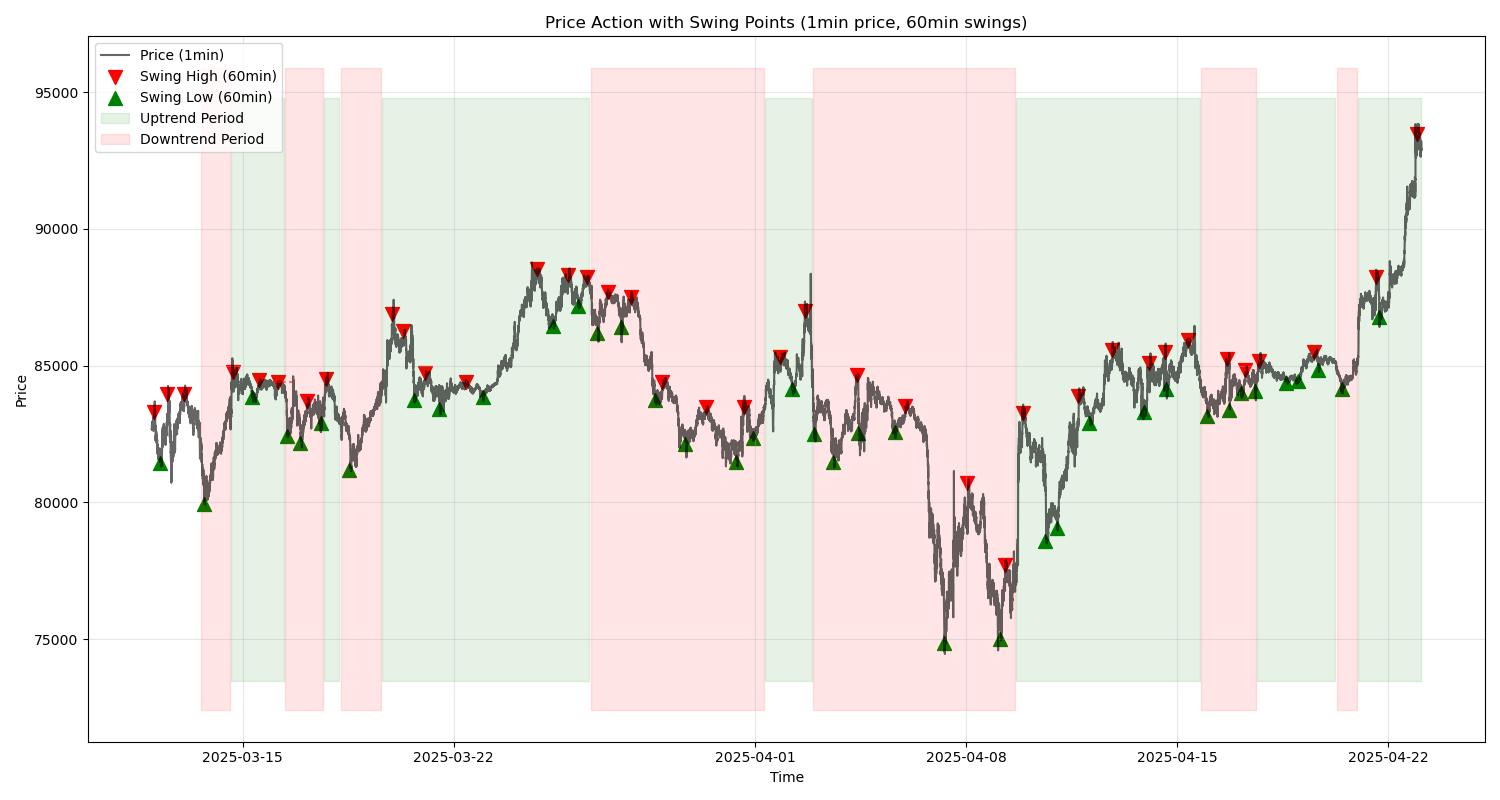
\includegraphics[width=\textwidth]{60min_swing_point_bias.png}
  \caption{1 min interval price with 60 min swing points and a $n$ value of 8}
\end{figure}



\newpage
\section*{Combining Indicators}
Here I visulised the swing points, the EMA spread and the 100 outliers with the highest Z-Score in the same plot.

\begin{figure}[H]
    \centering
    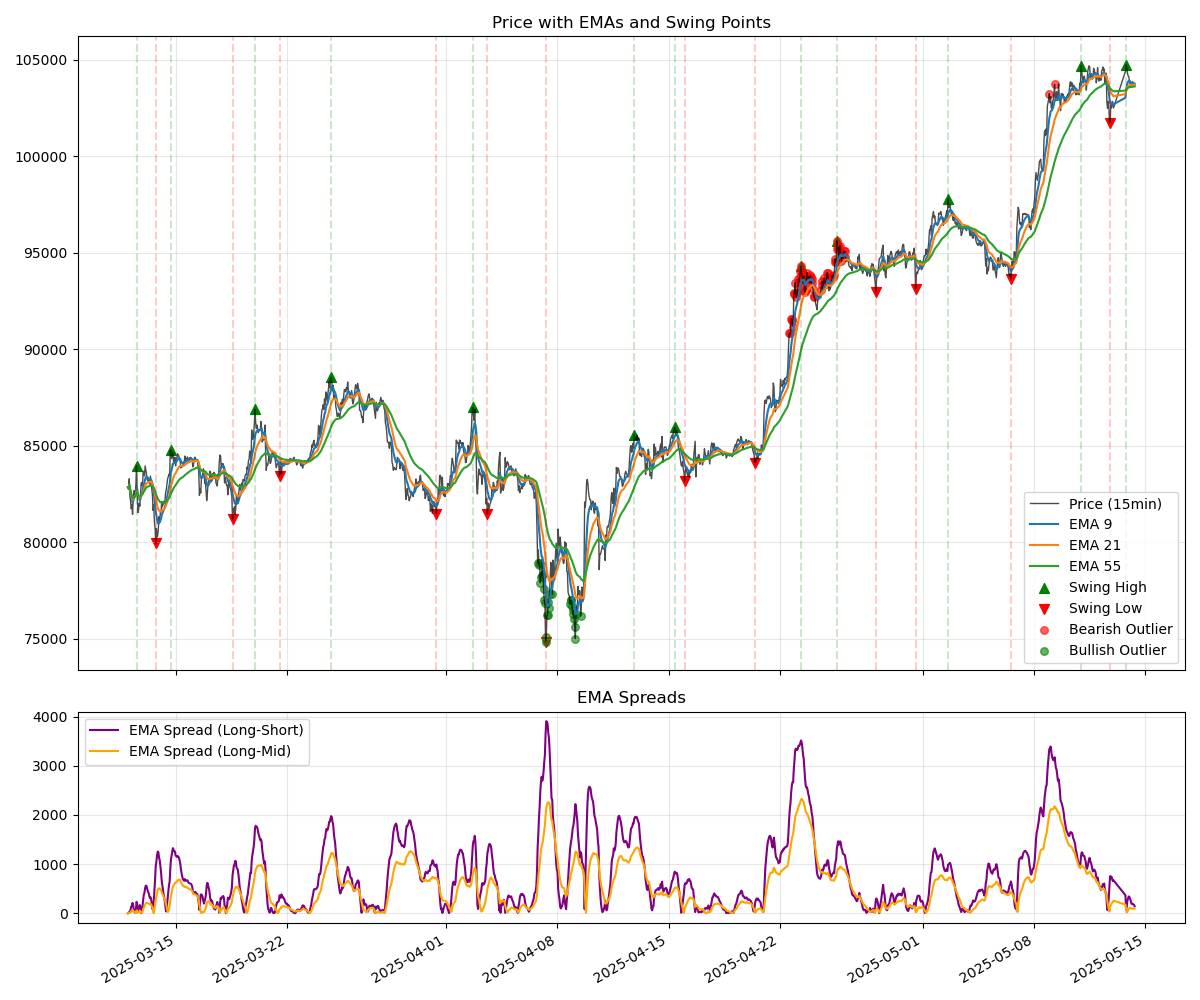
\includegraphics[width=\textwidth]{imgs/swingpoints_emaspread_priceOutliers.png}
    \caption{combined indicators png}
\end{figure}

\footnote{Chart made with Matplotlib and Seaborn}


\newpage
\section*{Mapping Orderbook delta EMA with standard deviation shifing}
\section*{Formulars}

\begin{equation}
  EMA_t = \alpha \cdot \Delta_t + (1 - \alpha) \cdot EMA_{t-1}
\end{equation}

Dictionary of Terms

\begin{itemize}
  \item $EMA_t$ - Exponential Moving Average at time $t$
  \item $\Delta_t$ - Orderbook delta at time $t$
  \item $\alpha$ - Smoothing factor
  \item $\sigma(\Delta)$ - Standard deviation of the orderbook delta with a 
\end{itemize}

We'll now shift the EMA by the standard deviation of the orderbook delta 





\newpage
\section*{sources}
\subsection*{\href{https://x.com/HangukQuant/status/1930603876069335120}{url}: How good or random is your trading}








\end{document}